%%==============================================================
%%  Artigo: guia e modelo abnTeX2 para trabalhos acadêmicos da UFV
%%  Formato: ABNT NBR 6022:2018, classe abntex2 (opção article)
%%  Citações e referências: abnt=2023 (NBR 10520:2023 + NBR 6023:2018)
%%==============================================================
\documentclass[
	article,
	12pt,
	oneside,
	a4paper,
	english,
	brazil,
]{abntex2}

\usepackage{lmodern}
\usepackage[T1]{fontenc}
\usepackage[utf8]{inputenc}
\usepackage{indentfirst}
\usepackage{graphicx}
\usepackage{booktabs}
\usepackage{array}
\newcolumntype{L}[1]{>{\raggedright\arraybackslash}p{#1}}
\usepackage{tikz}
\usetikzlibrary{arrows.meta,positioning,fit}
\usepackage{minted}

% Pacote da UFV, carregado por último; define a versão da ABNT
\usepackage[abnt=2023]{misc/abntex2-UFV}
\arquivoreferencias{referencias}
\setlength{\emergencystretch}{3em}

\titulo{Guia e modelo \LaTeX\ para trabalhos acadêmicos com escolha da edição das normas ABNT de citação e referência}
\tituloestrangeiro{A \LaTeX\ guide and template for academic works with selectable editions of the ABNT citation and reference standards}
\autor{Matheus Breguêz\thanks{E-mail: \href{mailto:matbrgz@gmail.com}{matbrgz@gmail.com}.}}
\local{Brasil}
\data{2026}

\makeatletter
\hypersetup{
	pdftitle={\@title},
	pdfauthor={Matheus Breguêz},
	pdfcreator={LaTeX with abnTeX2},
	colorlinks=true,
	linkcolor=black,
	citecolor=blue,
	urlcolor=blue
}
\makeatother

% Resumos logo após o título (NBR 6022)
\renewcommand{\maketitlehookd}{%
	\vspace{\onelineskip}
	\begin{resumoumacoluna}
		Trabalhos acadêmicos brasileiros seguem as normas da Associação Brasileira de Normas Técnicas, entre elas a NBR 6023, de referências, revista em 2018 e em 2025, e a NBR 10520, de citações, revista em 2023. Modelos \LaTeX\ costumam implementar uma única edição dessas normas, e a troca de edição exige substituir o sistema bibliográfico e reescrever os comandos de citação. Este artigo apresenta um projeto de código aberto, derivado de um modelo de trabalho de conclusão de curso da Universidade Federal de Viçosa, que reúne três contribuições: um pacote de estilo sobre a classe abn\TeX2 com uma opção para escolher a edição das normas de citação e referência, de modo que o mesmo texto compile segundo as edições de 2002, segundo a NBR 6023:2018 com a NBR 10520:2002 ou segundo a NBR 6023:2018 com a NBR 10520:2023; um guia-modelo em que cada capítulo explica uma parte do trabalho acadêmico e demonstra no próprio código como produzi-la; e um processo de compilação, verificação e distribuição que gera um pacote pronto para cada edição. A verificação compilou os dois modelos nas três configurações sem citações indefinidas e confirmou, nos documentos gerados, as diferenças previstas entre as edições, como a grafia do autor nas citações e a apresentação de endereços eletrônicos nas referências.

		\vspace{\onelineskip}
		\noindent
		\textbf{Palavras-chave}: ABNT; \LaTeX; abn\TeX2; trabalho acadêmico; normalização.
	\end{resumoumacoluna}

	\begin{otherlanguage*}{english}
	\begin{resumoumacoluna}[Abstract]
		Brazilian academic works follow the standards of the Brazilian Association of Technical Standards (ABNT), including NBR 6023, on references, revised in 2018 and 2025, and NBR 10520, on citations, revised in 2023. \LaTeX\ templates usually implement a single edition of these standards, and switching editions requires replacing the bibliography system and rewriting citation commands. This article presents an open-source project, derived from an undergraduate thesis template of the Federal University of Viçosa, with three contributions: a style package built on the abn\TeX2 class with an option to choose the edition of the citation and reference standards, so that the same text compiles according to the 2002 editions, to NBR 6023:2018 with NBR 10520:2002, or to NBR 6023:2018 with NBR 10520:2023; a guide-template in which each chapter explains one part of an academic work and shows in its own source code how to produce it; and a build, verification and distribution process that generates a ready-to-use package for each edition. The verification compiled both templates in the three configurations with no undefined citations and confirmed, in the generated documents, the expected differences between editions, such as the spelling of authors in citations and the presentation of web addresses in references.

		\vspace{\onelineskip}
		\noindent
		\textbf{Keywords}: ABNT; \LaTeX; abn\TeX2; academic writing; standardization.
	\end{resumoumacoluna}
	\end{otherlanguage*}
}

\begin{document}
\selectlanguage{brazil}
\frenchspacing
\maketitle

\textual

% ----------------------------------------------------------
\section{Introdução}\label{sec:introducao}
% ----------------------------------------------------------

A apresentação de trabalhos acadêmicos no Brasil é regida por um conjunto de normas da Associação Brasileira de Normas Técnicas (ABNT). A NBR 14724 define a estrutura de teses, dissertações e trabalhos de conclusão de curso \cite{abnt14724}; a NBR 6023, a elaboração de referências \cite{abnt6023}; e a NBR 10520, a apresentação de citações \cite{abnt10520}. Completam o conjunto normas sobre numeração progressiva \cite{abnt6024}, sumário \cite{abnt6027} e resumo \cite{abnt6028}.

Três dessas normas foram revistas recentemente. A NBR 6023 teve novas edições em 2018, que substituiu a de 2002 \cite{abnt6023-2002}, e em 2025 \cite{abnt6023-2025}; a NBR 10520 teve nova edição em 2023, que substituiu a de 2002 \cite{abnt10520-2002}; e a NBR 14724 teve nova edição em 2024. Durante a transição entre edições, convivem exigências diferentes: cursos, programas e orientadores podem adotar a edição vigente, manter a anterior ou combinar a NBR 6023 de 2018 com a NBR 10520 de 2002, situação que perdurou de 2018 a 2023.

O \LaTeX\ \cite{lamport1994}, construído sobre o \TeX\ \cite{knuth1984texbook}, é usado na escrita acadêmica porque separa o conteúdo da formatação e gera automaticamente numeração, sumário, listas, citações e referências \cite{mittelbach2004}. No Brasil, a classe abn\TeX2 \cite{abntex2classe,ctan-abntex2} implementa as normas da ABNT para trabalhos acadêmicos. As citações e referências, porém, dependem de um sistema bibliográfico à parte, e cada sistema disponível implementa edições diferentes das normas. Um modelo que adota um deles fica preso às edições que ele implementa.

Este artigo apresenta um projeto de código aberto \cite{modeloufv} que trata esse problema em três frentes:

\begin{alineas}
	\item um pacote de estilo, sobre a classe abn\TeX2, com uma opção que escolhe a edição das normas de citação e referência sem alterar o texto do documento;
	\item um guia-modelo, em que cada capítulo explica uma parte do trabalho acadêmico e demonstra, no próprio código-fonte, como produzi-la;
	\item um processo automatizado de compilação, verificação e distribuição, que gera um pacote pronto para cada edição.
\end{alineas}

O projeto deriva de um modelo de trabalho de conclusão de curso do curso de Sistemas de Informação da Universidade Federal de Viçosa (UFV), \textit{Campus} de Rio Paranaíba, cujo pacote de estilo data de 2014 e que foi publicado como repositório aberto em 2019.

A \autoref{sec:fundamentacao} apresenta as normas envolvidas e as ferramentas sobre as quais o projeto é construído. A \autoref{sec:projeto} descreve o projeto, e a \autoref{sec:verificacao}, a verificação realizada. A \autoref{sec:discussao} discute as limitações, e a \autoref{sec:conclusao} conclui o artigo.

% ----------------------------------------------------------
\section{Fundamentação}\label{sec:fundamentacao}
% ----------------------------------------------------------

\subsection{Edições das normas de citação e referência}

A NBR 10520 define os sistemas de chamada das citações e a forma de indicar autor, data e página. A principal mudança da edição de 2023 em relação à de 2002 está na grafia do autor dentro dos parênteses: na edição de 2002, o sobrenome é escrito em letras maiúsculas, como em (SILVA, 2020); na de 2023, em maiúsculas e minúsculas, como em (Silva, 2020), da mesma forma que fora dos parênteses \cite{abnt10520,abnt10520-2002}.

A NBR 6023 define os elementos e a ordem de apresentação das referências. Entre as diferenças visíveis da edição de 2018 em relação à de 2002 estão a forma das expressões para local e editora não identificados, que passam de [S.l.] e [s.n.] para \textit{[S. l.]} e \textit{[s. n.]}, e a apresentação do endereço eletrônico, que deixa de ser escrito entre os sinais \texttt{< >} \cite{abnt6023,abnt6023-2002}. A edição de 2025 alterou pontos específicos: os elementos das referências de coleções e fascículos de periódicos, de artigos eletrônicos, com a inclusão da e-localização, de eventos no todo e de jurisprudência \cite{abnt6023-2025}.

A NBR 14724, revista em 2024, manteve as regras de margens, fonte, espaçamento e paginação, e passou a determinar que o trabalho acadêmico seja organizado em seções, e não em capítulos \cite{abnt14724}.

\subsection{Ferramentas}

No \LaTeX, as referências são cadastradas em um arquivo no formato Bib\TeX, e um programa externo seleciona as obras citadas, ordena-as e as formata segundo um estilo. Há duas pilhas em uso com a classe abn\TeX2:

\begin{alineas}
	\item o pacote \texttt{abntex2cite} \cite{abntex2cite}, distribuído com a classe, que usa o programa Bib\TeX\ e implementa a NBR 6023 e a NBR 10520 de 2002;
	\item o pacote \texttt{biblatex} \cite{biblatex}, com o estilo \texttt{biblatex-abnt} \cite{biblatexabnt} e o programa Biber \cite{biber}; a versão 4.0 desse estilo implementa a NBR 6023:2018 e a NBR 10520:2023, mas não as alterações da NBR 6023:2025, e oferece a opção \texttt{accite}, que escreve o autor em maiúsculas nas citações, como na edição de 2002 da NBR 10520.
\end{alineas}

As duas pilhas diferem nos comandos de citação: o \texttt{abntex2cite} oferece \verb|\citeonline| para a citação com o autor integrado ao texto, e o \texttt{biblatex-abnt}, \verb|\textcite|. Também diferem no programa executado entre as compilações e na forma de declarar o arquivo de referências.

\subsection{Automação e reprodutibilidade}

Um documento \LaTeX\ é compilado como um programa, e práticas do desenvolvimento de software se aplicam à sua produção. Controle de versões, automação de tarefas repetitivas e verificação automática estão entre as práticas recomendadas para o trabalho científico com computadores \cite{wilson2014,wilson2017}. Registrar como cada resultado foi gerado e com quais versões de programas é condição para reproduzi-lo \cite{sandve2013}. O projeto aplica essas práticas ao próprio modelo: as versões são controladas com Git \cite{chacon2014}, a compilação é automatizada com o \texttt{latexmk} \cite{latexmk} e as versões publicadas seguem o versionamento semântico \cite{semver}.

% ----------------------------------------------------------
\section{O projeto}\label{sec:projeto}
% ----------------------------------------------------------

A \autoref{fig:arquitetura} resume a organização do projeto. O pacote de estilo e a base de referências têm uma única fonte, no diretório \texttt{estilo/}, e são copiados para cada modelo, de modo que cada modelo possa ser usado isoladamente, inclusive em editores on-line. O guia é escrito no modelo modular, e o modelo de arquivo único é gerado a partir dele. Cada modelo é compilado nas três configurações, e o resultado é empacotado para distribuição.

\begin{figure}[htbp]
	\caption{Organização do projeto e fluxo de compilação}\label{fig:arquitetura}
	\centering
	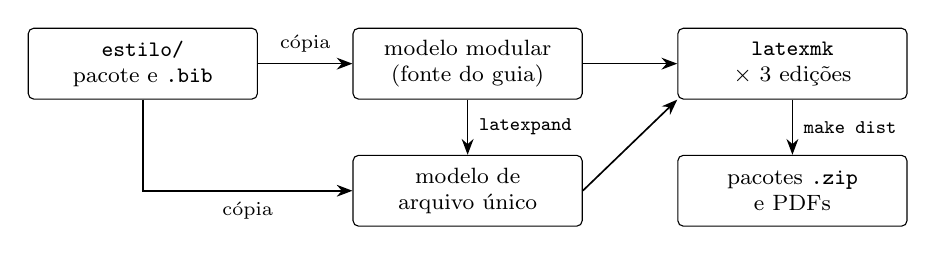
\begin{tikzpicture}[
		node distance=7mm and 6mm,
		caixa/.style={draw, rounded corners=2pt, align=center, font=\footnotesize, minimum height=9mm, text width=27mm, inner sep=3pt},
		seta/.style={-{Stealth[length=2mm]}, semithick},
		rotulo/.style={font=\scriptsize, midway, fill=white, inner sep=1pt}
	]
		\node[caixa] (estilo) {\texttt{estilo/}\\pacote e \texttt{.bib}};
		\node[caixa, right=12mm of estilo] (modular) {modelo modular\\(fonte do guia)};
		\node[caixa, below=of modular] (unico) {modelo de\\arquivo único};
		\node[caixa, right=12mm of modular] (latexmk) {\texttt{latexmk}\\$\times$ 3 edições};
		\node[caixa, below=of latexmk] (dist) {pacotes \texttt{.zip}\\e PDFs};
		\draw[seta] (estilo) -- node[rotulo, above=1mm] {cópia} (modular);
		\draw[seta] (estilo.south) |- node[rotulo, pos=0.75, below=1mm] {cópia} (unico.west);
		\draw[seta] (modular) -- node[rotulo, right=1mm] {\texttt{latexpand}} (unico);
		\draw[seta] (modular) -- (latexmk);
		\draw[seta] (unico.east) -- (latexmk.south west);
		\draw[seta] (latexmk) -- node[rotulo, right=1mm] {\texttt{make dist}} (dist);
	\end{tikzpicture}
	\fonte{Elaborado pelo próprio autor.}
\end{figure}

\subsection{Seleção da edição}

O pacote \texttt{abntex2-UFV} recebe a opção \texttt{abnt}, com três valores. O \autoref{qua:mapeamento} mostra a pilha bibliográfica que cada valor carrega.

\begin{quadro}[htbp]
	\caption{Valores da opção \texttt{abnt} e pilha bibliográfica correspondente}\label{qua:mapeamento}
	\centering
	\footnotesize
	\begin{tabular}{L{0.08\textwidth}L{0.2\textwidth}L{0.17\textwidth}L{0.41\textwidth}}
		\toprule
		\textbf{Valor} & \textbf{Citações} & \textbf{Referências} & \textbf{Pilha} \\
		\midrule
		\texttt{2023} & NBR 10520:2023 & NBR 6023:2018 & \texttt{biblatex-abnt} e Biber \\
		\texttt{2018} & NBR 10520:2002 & NBR 6023:2018 & \texttt{biblatex-abnt} com \texttt{accite} e Biber \\
		\texttt{2002} & NBR 10520:2002 & NBR 6023:2002 & \texttt{abntex2cite} e Bib\TeX \\
		\bottomrule
	\end{tabular}
	\fonte{Elaborado pelo próprio autor.}
\end{quadro}

Para que o mesmo texto compile com qualquer valor, o pacote oferece uma interface comum. No preâmbulo, \verb|\arquivoreferencias| declara a base de referências; nos elementos pós-textuais, \verb|\imprimirreferencias| imprime a lista. Na pilha \texttt{biblatex}, o pacote define \verb|\citeonline| e \verb|\apudonline| como sinônimos dos comandos equivalentes do \texttt{biblatex-abnt}, e os comandos \verb|\cite| e \verb|\apud| têm a mesma sintaxe nas duas pilhas. Um documento escrito para o \texttt{abntex2cite} passa, assim, a compilar também nas edições de 2018 e 2023. O uso no documento se reduz a:

\begin{minted}[fontsize=\footnotesize]{latex}
\usepackage[abnt=2023]{misc/abntex2-UFV}
\arquivoreferencias{referencias}
...
segundo \citeonline[p.~97]{knuth1984literate}, ...
...
\imprimirreferencias
\end{minted}

A edição também pode ser escolhida sem editar o documento: se a macro \verb|\ABNTversao| estiver definida antes do preâmbulo, ela tem precedência sobre a opção do pacote. O processo de compilação usa esse mecanismo para gerar as três configurações a partir do mesmo arquivo. Um valor inválido interrompe a compilação com uma mensagem que lista os valores aceitos.

O pacote ajusta ainda opções do \texttt{biblatex} para aproximar a saída da norma. A opção \texttt{extradate} repete na lista de referências a letra que distingue obras do mesmo autor e ano, como 1984a e 1984b. A opção \texttt{uniquelist=false} impede que o \texttt{biblatex} estenda a lista de autores para distinguir obras com o mesmo primeiro autor, o que produziria citações como (Wilson; Aruliah \textit{et al.}, 2014) em vez de (Wilson \textit{et al.}, 2014).

\subsection{Guia-modelo}

O conteúdo do modelo é, ao mesmo tempo, um guia. Cada capítulo trata de uma parte do trabalho acadêmico e demonstra, no próprio texto, o recurso que descreve: a estrutura do trabalho e as regras de formatação da NBR 14724; a numeração progressiva até a seção quinária; os tipos de citação, com supressões, destaques, citação de citação e notas; a elaboração de referências para doze tipos de documento; ilustrações, tabelas no padrão do IBGE \cite{ibge1993}, quadros, equações, algoritmos e código-fonte \cite{minted}; e as ferramentas de compilação, gestão de referências e controle de versões. As referências de exemplo são documentos reais, para que o leitor possa conferir cada referência gerada com a obra correspondente.

O guia é escrito no modelo modular, com um arquivo por capítulo. O modelo de arquivo único, preferido por quem começa a usar \LaTeX, é gerado a partir do modular pelo \texttt{latexpand} \cite{latexpand}, que expande os comandos de inclusão de arquivos. Assim, os dois modelos têm o mesmo conteúdo, e só um deles é editado.

\subsection{Compilação, verificação e distribuição}

Um \texttt{Makefile} concentra as operações do projeto. O alvo \texttt{todas} compila os dois modelos nas três configurações, executando o \texttt{latexmk} com a macro \verb|\ABNTversao| definida para cada edição; o \texttt{latexmk} identifica se a configuração usa Bib\TeX\ ou Biber. O alvo \texttt{check} executa as verificações:

\begin{alineas}
	\item as cópias do pacote e da base de referências em cada modelo são idênticas às fontes em \texttt{estilo/};
	\item o modelo de arquivo único é idêntico ao gerado a partir do modular;
	\item a compilação com uma edição inexistente falha com o erro do pacote, e não por outro motivo;
	\item os dois modelos compilam nas três configurações.
\end{alineas}

O alvo \texttt{dist} gera, para cada modelo e cada edição, um arquivo compactado com o código-fonte já configurado para aquela edição e o PDF correspondente. Um fluxo de integração contínua é configurado para executar \texttt{check} e \texttt{dist} a cada alteração e, quando uma versão é marcada no repositório, anexa os pacotes à página de publicação. Quem não usa linha de comando escolhe a edição ao baixar o pacote.

% ----------------------------------------------------------
\section{Verificação}\label{sec:verificacao}
% ----------------------------------------------------------

A verificação foi feita com o \TeX\ Live 2026, \texttt{latexmk} 4.88, \texttt{biblatex} 3.21, Biber 2.21, \texttt{biblatex-abnt} 4.0 e abn\TeX2 1.9.7. Os dois modelos foram compilados nas três configurações, num total de seis documentos, com 40 páginas cada. Em todos, o registro de compilação não apresentou citações ou referências cruzadas indefinidas nem linhas que ultrapassam a margem, e a compilação com uma edição inexistente foi interrompida pelo erro do pacote.

Para conferir se a opção produz as diferenças previstas pelas normas, foram extraídos dos documentos gerados os mesmos trechos nas três configurações. O \autoref{qua:saidas} reproduz esses trechos.

\begin{quadro}[htbp]
	\caption{Trechos dos documentos gerados em cada configuração}\label{qua:saidas}
	\centering
	\footnotesize
	\begin{tabular}{L{0.07\textwidth}L{0.14\textwidth}L{0.24\textwidth}L{0.41\textwidth}}
		\toprule
		\textbf{Valor} & \textbf{Citação} & \textbf{Citação com página} & \textbf{Referência de página da internet (trecho)} \\
		\midrule
		\texttt{2002} & (GIL, 2017) & (KNUTH, 1984b, p.~97) & 2013. Disponível em: \texttt{<https://semver.org/lang/pt-BR/>}. \\
		\texttt{2018} & (GIL, 2017) & (KNUTH, 1984a, p.~97) & \textit{[S. l.: s. n.]}, 2013. Disponível em: \texttt{https://semver.org/lang/pt-BR/}. \\
		\texttt{2023} & (Gil, 2017) & (Knuth, 1984a, p.~97) & \textit{[S. l.: s. n.]}, 2013. Disponível em: \texttt{https://semver.org/lang/pt-BR/}. \\
		\bottomrule
	\end{tabular}
	\fonte{Elaborado pelo próprio autor a partir dos documentos gerados.}
\end{quadro}

Os trechos confirmam as diferenças descritas na \autoref{sec:fundamentacao}. A grafia do autor nas citações muda apenas na configuração 2023, que é a única a seguir a NBR 10520:2023. As configurações 2018 e 2023, que seguem a NBR 6023:2018, apresentam o endereço eletrônico sem os sinais \texttt{< >} e indicam local e editora não identificados; a configuração 2002 mantém os sinais.

A verificação também revelou diferenças que não decorrem das normas, mas das implementações. A letra que distingue as duas obras de Knuth publicadas em 1984 é atribuída de forma diferente pelas duas pilhas: a mesma obra recebe 1984b na configuração 2002 e 1984a nas demais, porque cada pilha ordena de um modo as obras do mesmo autor e ano. Além disso, o \texttt{abntex2cite} acrescenta a letra apenas na citação, enquanto o \texttt{biblatex-abnt}, com a opção \texttt{extradate}, acrescenta-a também na lista de referências. Antes do ajuste da opção \texttt{uniquelist}, a mesma verificação mostrou a citação com dois autores antes de \textit{et al.}, descrita na \autoref{sec:projeto}. A inspeção dos documentos também mostrou que o ambiente de quadro perdia a formatação quando o pacote \texttt{float}, carregado por outros pacotes, era lido antes do pacote de estilo, porque o \texttt{float} substitui o comando do \textit{memoir} que cria novos tipos de flutuante; o pacote passou a definir o quadro sem depender desse comando.

% ----------------------------------------------------------
\section{Discussão e limitações}\label{sec:discussao}
% ----------------------------------------------------------

A opção do pacote altera apenas citações e referências. A estrutura e a formatação do trabalho seguem a NBR 14724:2024, cujas regras de layout coincidem com as da edição anterior implementada pela classe abn\TeX2; para atender à exigência de organização em seções, o pacote faz os cabeçalhos e as referências cruzadas dizerem ``Seção'' em vez de ``Capítulo''. A numeração progressiva segue a NBR 6024 de 2012, e o layout é o mesmo nas três configurações. A configuração intermediária, que combina a NBR 6023:2018 com a NBR 10520:2002, corresponde ao período entre as duas revisões e atende a regulamentos que ainda o adotam.

A conformidade das referências com as normas depende dos estilos bibliográficos usados. O projeto não reimplementa as normas; ele seleciona e ajusta implementações existentes. A verificação descrita na \autoref{sec:verificacao} confere, por inspeção dos documentos gerados, um conjunto de diferenças conhecidas entre as edições, e não substitui uma validação sistemática contra o texto das normas. Diferenças entre as implementações, como a atribuição das letras do ano, permanecem nos documentos gerados.

Nenhuma das configurações implementa a NBR 6023:2025. Como as alterações dessa edição se restringem a alguns tipos de documento, o guia indica esses tipos para que o autor confira as referências correspondentes; incorporar a edição de 2025 exige um estilo bibliográfico que a implemente e um novo valor da opção.

Duas dependências merecem registro. A última versão da classe abn\TeX2 e do pacote \texttt{abntex2cite} é de 2018 \cite{ctan-abntex2}, de modo que a configuração 2002 depende de um código sem manutenção ativa. E o pacote \texttt{minted}, usado no guia para o realce de código-fonte, exige o Python instalado, o que acrescenta um requisito para quem compila o modelo localmente; o guia indica como removê-lo quando não for necessário.

% ----------------------------------------------------------
\section{Conclusão}\label{sec:conclusao}
% ----------------------------------------------------------

O artigo apresentou um projeto que permite escrever um trabalho acadêmico em \LaTeX\ uma única vez e gerá-lo segundo três combinações de edições das normas ABNT de citação e referência. Um pacote sobre a classe abn\TeX2 oferece uma interface comum aos dois sistemas bibliográficos disponíveis; um guia-modelo demonstra no próprio texto os recursos de que um trabalho acadêmico precisa; e um processo automatizado compila, verifica e distribui os modelos em cada configuração.

A verificação mostrou que os documentos gerados apresentam as diferenças previstas entre as edições e expôs diferenças entre as implementações, parte das quais foi corrigida por opções do pacote. O mesmo mecanismo de seleção pode ser estendido a novas edições das normas, acrescentando um valor à opção e o estilo bibliográfico correspondente. O projeto está disponível sob a licença MIT \cite{modeloufv}.

% ----------------------------------------------------------
% Elementos pós-textuais
% ----------------------------------------------------------
\postextual

\section*{Agradecimentos}
\addcontentsline{toc}{section}{Agradecimentos}

A Rodrigo Smarzaro, autor do modelo de trabalho de conclusão de curso que deu origem ao projeto, e ao Centro Acadêmico de Sistemas de Informação da Universidade Federal de Viçosa, \textit{Campus} de Rio Paranaíba, em cuja organização o projeto é mantido.

\imprimirreferencias

\end{document}
